\documentclass[11pt,letterpaper]{article}
\input{G:/Dropbox/Math/preamble}
\usepackage{fullpage}
\usepackage{multicol}
\everymath{\displaystyle}

\begin{document}
\flushleft
\begin{multicols}{2}

\begin{large}\textbf{Math 2554 Exam 2: Sections 3.9-4.5 \\
Fri 7 Nov 2014}\end{large}

\hfill\textbf{Name:  }\underline{\hspace{40ex}} %KEY\hspace{17ex}} 
\\
\vspace{.5in}

\end{multicols}

\pagestyle{empty}

\flushleft

\begin{center}\Large Calculus I 

Exam 2 \end{center}

\vspace{2pc}
Please provide the following data:

\vspace{2pc}
Drill Instructor: \underline{\hspace{40ex}}

\vspace{2pc}
Drill Time: \underline{\hspace{40ex}}

\vspace{2pc}
Student ID or clicker \#: \underline{\hspace{40ex}}

\vspace{3pc}
{\bf Exam Instructions:} Sit with your drill section, according to the map shown on the projector.  You have 50 minutes to complete this exam.  One $3\times 5$ inch notecard, one side only, is allowed.  No graphing calculators.  No programmable calculators.  No electronic devices except for the approved calculators (so no phones, iDevices, computers, etc).  If you finish early then you may leave, UNLESS there are less than 5 minutes of class left.  To prevent disruption, if you finish with less than 5 minutes of class remaining then please stay seated and quiet.

\vspace{5pc}
Your signature below indicates that you have read this page and agree to follow the Academic Honesty Policies of the University of Arkansas.  

\vspace{3pc}
Signature: (1 pt) \underline{\hspace{80ex}}

\vfill
\begin{flushright}\Large Good luck!\end{flushright}

\begin{enumerate}
\newpage

\item Fill in the blanks for the following limit laws.
\begin{enumerate}
\item {\bf Quotients of Functions} 
\[\lim_{x\to a}\frac{f(x)}{g(x)}=\frac{\displaystyle\lim_{x\to a}f(x)}{\displaystyle\lim_{x\to a}g(x)}\] 

provided (1 pt) \underline{\hspace{20ex}}.  

\vspace{2pc}
(1 pt) If $g$ is a polynomial, then why is it OK to just require $g(a)\neq 0$ (instead of the limit at $a$)?

\vspace{5pc}
\item {\bf Fractional Powers} 
\[\lim_{x\to a}f(x)^{\frac{m}{n}}=\left(\lim_{x\to a}f(x)\right)^{\frac{m}{n}}\] 

provided $m,n>0$ are integers and $\frac{m}{n}$ is in lowest terms.  If $n$ is even, then we also need  (2 pts) \underline{\hspace{20ex}} for (1 pt) \underline{\hspace{30ex}}.  

\vspace{5pc}
Rewrite the rule for one-sided limits:
\[\lim_{x\to a^+}f(x)^{\frac{m}{n}}=\text{ (1 pt) \underline{\hspace{20ex}}}\]
provided $m,n>0$ are integers and $\frac{m}{n}$ is in lowest terms.  If $n$ is even, then we also need  (2 pts) \underline{\hspace{20ex}} for (2 pts) \underline{\hspace{30ex}}.   

\vspace{3pc}
\[\lim_{x\to a^-}f(x)^{\frac{m}{n}}=\text{ (1 pt) \underline{\hspace{20ex}}}\]
provided $m,n>0$ are integers and $\frac{m}{n}$ is in lowest terms.  If $n$ is even, then we also need  (2 pts) \underline{\hspace{20ex}} for (2 pts) \underline{\hspace{30ex}}.   

\newpage
\item {\bf End Behavior and Asymptotes of Rational Functions}

Suppose $f(x)=\frac{p(x)}{q(x)}$ is a rational function, and we write $p,q$ as
\begin{align*}p(x) & =a_mx^m+a_{m-1}x^{m-1}+\dots+a_2x^2+a_1x+a_0 \\
q(x) &=b_nx^n+b_{n-1}x^{n-1}+\dots+b_2x^2+b_1x+b_0
\end{align*}
with $a_m,b_n\neq 0$.

\vspace{1pc}
If $m<n$, then $\lim_{x\to\pm\infty}f(x)=$ (1 pt) \underline{\hspace{20ex}}, and (2 pts) \underline{\hspace{20ex}} is a horizontal asymptote for $f$.

\vspace{1pc}
If $m=n$, then $\lim_{x\to\pm\infty}f(x)=$  (1 pt) \underline{\hspace{20ex}}, and (2 pts) \underline{\hspace{20ex}} is a horizontal asymptote of $f$.

\vspace{1pc}
If $m>n$, then $\lim_{x\to\pm\infty}f(x)=$ (1 pt) \underline{\hspace{20ex}} or (1 pt) \underline{\hspace{20ex}}.

\end{enumerate}

\vspace{5pc}
\item For the following questions, if a one-sided limit is computed, your justification must involve determining the sign of the numerator and denominator for $x$-values sufficiently close to 0.

\begin{center}Suppose $g(x)=\begin{cases}\frac{x-5}{x} & x\neq 0 \\
	0 & x=0 \end{cases}$.\end{center}
	
Evaluate: 
\begin{enumerate}
\item (4 pts) $\lim_{x\to 0^+}g(x)$  

\vspace{5pc}
\item (4 pts) $\lim_{x\to 0^-}g(x)$  

\vspace{5pc}
\item (3 pts) $\lim_{x\to 0}g(x)$

\vspace{5pc}
\item (1 pt) $g(0)$
\end{enumerate}

\vspace{3pc} 
(2 pts) Does $g$ have a vertical asymptote at the line $x=0$?  Explain why or why not.

\vspace{5pc}
\begin{center}Now suppose $h(x)=\begin{cases}g(x) & x< 0 \\
	0 & x\geq 0 \end{cases}$.  \end{center}
	
Evaluate: 
\begin{enumerate}
\item (2 pts) $\lim_{x\to 0^+}h(x)$

\vspace{5pc} 
\item (3 pts) $\lim_{x\to 0^-}h(x)$  

\vspace{5pc}
\item (2 pts) $\lim_{x\to 0}h(x)$

\vspace{5pc}	
\item (1 pt) $h(0)$

\end{enumerate}
\vspace{3pc}
(2 pts) Does $h$ have a vertical asymptote at the line $x=0$?  Explain why or why not.

\newpage
\item (8 pts) Using Figure \ref{fig:pic2} as a guide, explain how the Squeeze Theorem can be used to compute 
\[\lim_{x\to 0}x^2\sin\left(\frac{1}{x}\right),\] 
and then say what the limit is.
\vspace{-1pc}  
\begin{figure}[h]
\begin{center}
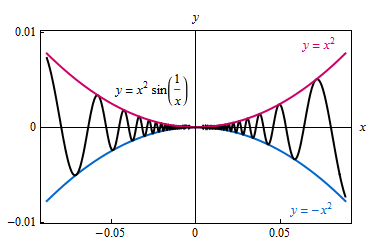
\includegraphics[scale=0.8]{Exam1pic2.png}
\caption{(Briggs, W. and Cochran, L. \emph{Calculus: Early Transcendentals})}\label{fig:pic2}
\end{center}
\end{figure}

\newpage
\item Given the graph of $f$ in the following figures, find the slope of the secant line that passes through $(0,0)$ and $(h,f(h))$, in terms of $h$.  Then calculate the limit of that slope as $h\to 0^+$ and as $h\to 0^-$.  
\begin{enumerate}
\item (5 pts) $f(x)=x^{\frac{1}{3}}$
\vspace{-1pc}  
\begin{figure}[h]
\begin{center}
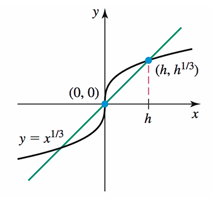
\includegraphics{Exam1pic4.png}
\caption{(Briggs, W. and Cochran, L. \emph{Calculus: Early Transcendentals})}
\end{center}
\end{figure}

\newpage
\item (5 pts) $f(x)=x^{\frac{2}{3}}$
\vspace{-1pc}  
\begin{figure}[h]
\begin{center}
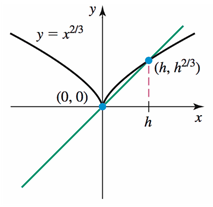
\includegraphics{Exam1pic5.png}
\caption{(Briggs, W. and Cochran, L. \emph{Calculus: Early Transcendentals})}
\end{center}
\end{figure}

\newpage
\item (4 pts) In both parts (a) and (b), what does your answer tell you about the tangent line to the curve at $(0,0)$?  Why doesn't $f$ itself have a vertical asymptote in either of these cases?

\end{enumerate}

\vspace{20pc}
\item (ChAlLeNgE pRoBlEm) Suppose $\lim_{x\to 1}f(x)=4$.  What is $\lim_{x\to -1}f(x^2)$? 

\newpage
\item For each function $f(x)$, evaluate $\lim_{x\to\infty}f(x)$ and $\lim_{x\to -\infty}f(x)$, and then identify any horizontal asymptotes.  Next, find the vertical asymptotes.  For each vertical asymptote $x=a$, evaluate $\lim_{x\to a^-}f(x)$ and $\lim_{x\to a^+}f(x)$.  Justify your answers.

\vspace{2pc}
\begin{enumerate}
\item (7 pts) $f(x)=\frac{x^2-4x+3}{x-1}$

\vspace{15pc}
\item (7 pts) $f(x)=\frac{x^2-4}{x(x-2)}$
\end{enumerate}

\newpage
\item (5 pts) Let $f(x)=x^2+5x-3$.  Evaluate, analytically:
\[\lim_{x\to 4}\frac{f(x)-f(4)}{x-4}\]

\vspace{20pc}
(3 pts) Use your answer above to write the equation of the tangent line to $f(x)$ at $x=4$.

\newpage
\item (6 pts) Does the function 
\[f(x)=2x^5-8x^3+5x^2+3x-5\] 
cross the horizontal line $y=-4$ for some $x$ in the interval $\left[0,1\right]$?  (Yes, it does.)  Justify your answer, and in particular, mention any important theorems you use and why they apply in this situation. 

\end{enumerate}

\end{document}


